\documentclass[12pt,]{article}
\usepackage{lmodern}
\usepackage{amssymb,amsmath}
\usepackage{ifxetex,ifluatex}
\usepackage{fixltx2e} % provides \textsubscript
\ifnum 0\ifxetex 1\fi\ifluatex 1\fi=0 % if pdftex
  \usepackage[T1]{fontenc}
  \usepackage[utf8]{inputenc}
\else % if luatex or xelatex
  \ifxetex
    \usepackage{mathspec}
  \else
    \usepackage{fontspec}
  \fi
  \defaultfontfeatures{Ligatures=TeX,Scale=MatchLowercase}
    \setmainfont[]{Arial}
\fi
% use upquote if available, for straight quotes in verbatim environments
\IfFileExists{upquote.sty}{\usepackage{upquote}}{}
% use microtype if available
\IfFileExists{microtype.sty}{%
\usepackage{microtype}
\UseMicrotypeSet[protrusion]{basicmath} % disable protrusion for tt fonts
}{}
\usepackage[margin=1in]{geometry}
\usepackage{hyperref}
\hypersetup{unicode=true,
            pdftitle={Seed plant families with diverse mycorrhizal states have higher diversification rates},
            pdfauthor={María Isabel Mujica1,2, María Fernanda Pérez1,2, Gustavo Burin3, Tiago Quental3},
            pdfborder={0 0 0},
            breaklinks=true}
\urlstyle{same}  % don't use monospace font for urls
\usepackage{graphicx,grffile}
\makeatletter
\def\maxwidth{\ifdim\Gin@nat@width>\linewidth\linewidth\else\Gin@nat@width\fi}
\def\maxheight{\ifdim\Gin@nat@height>\textheight\textheight\else\Gin@nat@height\fi}
\makeatother
% Scale images if necessary, so that they will not overflow the page
% margins by default, and it is still possible to overwrite the defaults
% using explicit options in \includegraphics[width, height, ...]{}
\setkeys{Gin}{width=\maxwidth,height=\maxheight,keepaspectratio}
\IfFileExists{parskip.sty}{%
\usepackage{parskip}
}{% else
\setlength{\parindent}{0pt}
\setlength{\parskip}{6pt plus 2pt minus 1pt}
}
\setlength{\emergencystretch}{3em}  % prevent overfull lines
\providecommand{\tightlist}{%
  \setlength{\itemsep}{0pt}\setlength{\parskip}{0pt}}
\setcounter{secnumdepth}{0}
% Redefines (sub)paragraphs to behave more like sections
\ifx\paragraph\undefined\else
\let\oldparagraph\paragraph
\renewcommand{\paragraph}[1]{\oldparagraph{#1}\mbox{}}
\fi
\ifx\subparagraph\undefined\else
\let\oldsubparagraph\subparagraph
\renewcommand{\subparagraph}[1]{\oldsubparagraph{#1}\mbox{}}
\fi

%%% Use protect on footnotes to avoid problems with footnotes in titles
\let\rmarkdownfootnote\footnote%
\def\footnote{\protect\rmarkdownfootnote}

%%% Change title format to be more compact
\usepackage{titling}

% Create subtitle command for use in maketitle
\providecommand{\subtitle}[1]{
  \posttitle{
    \begin{center}\large#1\end{center}
    }
}

\setlength{\droptitle}{-2em}

  \title{Seed plant families with diverse mycorrhizal states have higher
diversification rates}
    \pretitle{\vspace{\droptitle}\centering\huge}
  \posttitle{\par}
    \author{María Isabel Mujica\textsuperscript{1,2}, María Fernanda
Pérez\textsuperscript{1,2}, Gustavo Burin\textsuperscript{3}, Tiago
Quental\textsuperscript{3}}
    \preauthor{\centering\large\emph}
  \postauthor{\par}
    \date{}
    \predate{}\postdate{}
  
\usepackage[left]{lineno}
\linenumbers
\usepackage{setspace}
\doublespacing

\begin{document}
\maketitle

\textsuperscript{1} Departamento de Ecología, Pontificia Universidad
Católica de Chile, Santiago, Chile. \textsuperscript{2} Instituto de
Ecología y Biodiversidad (IEB), Santiago, Chile. \textsuperscript{3}
Departamento de Ecologia, Instituto de Biociências, Universidade de São
Paulo, 11294, 05422-970 São Paulo, Brazil.

\hypertarget{abstract}{%
\section{Abstract}\label{abstract}}

One crucial innovation in plant evolution was the association with soil
fungi during land colonization. Today, this symbiotic interaction is
present in most of plants species and can be classified in four types:
Arbuscular (AM), Ecto (EM), Orchid (OM) and Ericoid Mycorrhiza (ER).
Since the AM ancestral state, some plants lineages have switched partner
(EM, OM and ER) or lost the association (no-association: NM).
Evolutionary transitions to a novel mycorrhizal state (MS) might allow
plant lineages to access new resources, enhancing diversification rates.
However, some clades are not restricted to one MS, and this variability
might promote diversification. In this study we address the relationship
between MS and plant diversification rates of seed plant families. For
this, we compiled a database for \textasciitilde6400 seed plant species
and their mycorrhizal partners. We assigned a single MS to each plant
family, then calculated the heterogeneity of MS and estimated their
diversification rates using the method-of-moments. Families with mixed
MS had the highest diversification rates and there was a positive
relationship between heterogeneity of MS and diversification rates.
These results support the hypothesis that MS plasticity promotes
diversification and highlight the importance of the association with
soil fungi for the diversification of plants. Keywords: diversification
rates, mycorrhizal states, seed plants, key innovation, mycorrhizal
diversity

\hypertarget{introduction}{%
\section{Introduction}\label{introduction}}

Understanding the basis of the exceptional plant diversity has been a
matter of interest for ecologist and evolutionary biologist since
Darwin. Great focus has been placed on estimating plants diversification
rates and identifying the factors that could influence them (Eriksson \&
Bremer, 1992; Moore \& Donoghe, 2007; O´Meara et al., 2016; Vamosi et
al., 2018). The acquisition of novel traits (sometimes referred to as
``key innovations''), such as pollination by animals (Eriksson \&
Bremer, 1992) or physiological seed dormancy (Willis et al., 2014), have
been proposed to promote diversification of plant lineages. This ``key
innovation'' perspective suggests that the acquisition of a novel trait
might allow a given lineage to exploit the environment in a
significantly different way, potentially resulting in an explosive
radiation.

One crucial innovation in plants evolution was the association with soil
fungi during land colonization (Pirozynski \& Malloch, 1975; Selosse \&
Le Tacon, 1998). Before plant colonization, land was hostile, with
extreme drought and temperatures, and barren rocky substrate; hence, the
association with terrestrial fungi allowed the algae ancestors of plants
to successfully colonize the land (Selosse et al., 2015). This initial
symbiotic association was the prelude of modern mycorrhizas (Feijen et
al., 2018), the association between fungi and root plants in which
plants transfer carbon to fungi and receive nutrients in turn (Smith \&
Read, 2008). Today, this symbiosis is present in 86\% of land plants
species (van der Heijden et al., 2015), and based on their structure and
function can be classified in four major types: arbuscular mycorrhiza
(AM), ectomycorrhiza (EM), orchid mycorrhizal (OM) and ericoid
mycorrhizal (ER) (Brundrett, 2002).

Ancestral state reconstruction and the fossil record show that the
ancestor of seed plants probably had AM associations (Redecker et al.,
2002; Maherali et al., 2016). This is the most frequent mycorrhizal type
in plants (74\% of extant plant species) and is characterized by an
association with Glomeromycete fungi (van der Heijden et al., 2015).
Between 100 and 200 million years ago, some lineages switched fungal
partners to several lineages of Basidiomycetes, forming what is
described as the EM associations (Brundrett, 2002). The acquisition of
EM resulted in new root functional capabilities as freezing tolerance
(Lehto et al., 2008), which seem related to the dominance of EM
angiosperms and gymnosperm in cool forests (Brundrett, 2002). Similarly,
Orchidaceae and species within the Ericaceae family recruited new fungal
lineages and formed OM and ER associations respectively. Orchids
associate with fungal families Ceratobasidiaceae, Tulasnellaceae and
Sebacinaceae, which in addition to nutrient exchange, promote seed
germination which cannot germinate without mycorrhizal support
(Rasmussen, 2002). Ericoid mycorrhizal associations (ER), on the other
hand, involve mainly fungi from Sebacinales and Helotiales and are
mostly frequent under acidic and infertile heathland conditions (Perotto
et al., 2002; van der Heijden et al., 2015). Finally, some lineages have
lost their mycorrhizal associations and became non-mycorrhizal (NM).
This transition has frequently occurred through an intermediate state of
facultative arbuscular mycorrhiza (AM) plants (Maherali et al., 2016).
Some of NM lineages evolved alternative resource-acquisition strategies
(Werner et al., 2018) like cluster-roots in Proteaceae (Neumann \&
Martinoia, 2002) or parasitism in Loranthaceae (Wilson \& Calvin, 2006).

Therefore, since the AM ancestral state some plant lineages have
followed different mycorrhizal evolutionary pathways: switching partner
(EM, OM and ER) or losing the association (Werner et al., 2018).
Evolutionary transitions to a novel mycorrhizal state might allow plant
lineages to access unexplored ecological resources, facilitating them to
colonize environments that were not available before, and possibly
enhancing their diversification rates. However, there are lineages in
which some species acquire a new mycorrhizal state and at the same time,
other species retain the ancestral state (AM) (Brundrett, 2008)
increasing the variability of mycorrhizal states, which might in fact
promote diversification of these lineages. Both hypotheses have not been
evaluated in plants; however the few studies available from the fungal
perspective suggest that shifts in mycorrhizal associations might affect
diversification of involved partners (Sánchez-García \& Matheny, 2017;
Sato et al., 2017).

Even though mycorrhizal symbiosis has been pointed out as a key factor
in the evolution and diversification of land plants (Brundrett \&
Tedersoo, 2018a; Feijen et al., 2018) this has not been evaluated
before. In this study we address the following questions: (1) Do the
lineages that established derived mycorrhizal associations present
higher diversification rates than the ones that retain the ancestral
mycorrhizal state? This investigates the idea of a key innovation
mechanism of diversification; (2) Is there a relationship between
mycorrhizal variability and diversification rates among different plant
lineages? This would investigate the idea that evolutionary lability
might increase diversification dynamics. To answer these questions, we
explored the relationship between the mycorrhizal state and the
diversification rates of several seed plant families.

\hypertarget{materials-and-methods}{%
\section{Materials and Methods}\label{materials-and-methods}}

\hypertarget{mycorrhizal-state-database}{%
\subsection{Mycorrhizal state
database}\label{mycorrhizal-state-database}}

We used the species-level dataset of mycorrhizal status from Maherali et
al., (2016), which compiles previous lists and surveys of plant species
and their mycorrhizal associations. Then, to increase sample size, we
reviewed publications that report mycorrhizal states for single species,
species list or local vegetation. Our literature compilation resulted in
a database of 6440 plant seed species and their mycorrhizal state
(Supporting Information, Notes S1). We used Maherali et al., (2016)
classification, and assigned species into one of these categories:
arbuscular mycorrhizal (AM), ectomycorrhiza (EM) Orchid mycorrhizal
(OM), Ericoid mycorrhizal (ER) and Non-mycorrhizal (NM). Species that
were characterized as AMNM by Maherali et al., (2016) - i.e.~species
observed as AM in some environments and NM in others- were here
considered as AM as they correspond to facultative AM species. Also, as
Maherali et al., (2016), species that formed both AM and EM, were placed
in the EM category to account species that were potentially capable of
forming EM symbiosis. The species names were reviewed using the
Taxonomic Name Resolution Service (Boyle et al., 2013). Recently,
Brundrett \& Tedersoo (2018b) pointed out potential mistakes in
mycorrhizal type identification on large databases, and how these
misdiagnoses might lead to wrong conclusions. For the case of Maherali
et al., (2016) database, the authors estimated an error in 1.6\% genera
and 1.0\% species,. Moreover, their approach used to determine these
errors (taxonomic approach; Brundrett, 2017) is controversial (Bueno et
al., 2018; Bueno et al., 2019; Sun et al., 2019). Nevertheless, to
assess the effect of possible undetected errors in the mycorrhizal
dataset, we introduced error to the mycorrhizal state by changing
mycorrhizal type at random of 20\% of plant species (one order of
magnitude higher than the error estimated from Brundrett \& Tedersoo
2018b) and obtained similar results to those derived from original data
(Supporting Information, Table S1).

\hypertarget{family-mycorrhizal-state-and-diversity}{%
\subsection{Family mycorrhizal state and
diversity}\label{family-mycorrhizal-state-and-diversity}}

We obtained information for species belonging to 259 seed plant
families, although the species sampling among families was highly
variable. To reduce the chance of wrongly assigning a family mycorrhizal
state, we considered those families for which we had either 5\% or
higher of species sampled or at least 8 species sampled. This is
justified because although many families are species-rich, they also
seem to be quite consistent with respect to mycorrhizal association
(Brundrett, 2008). This reduced our dataset to 175 families. Each family
was assigned a unique mycorrhizal state (AM, EM, NM, ER or OM) when more
than 60\% of species sampled belonged to this mycorrhizal state. If no
single state were present in more than 60\% of species, the family was
assigned a ``mixed'' state, to indicate no dominance of any mycorrhizal
association. Other thresholds for the assignment of family mycorrhizal
state were tested and the pattern was similar (50\%, 80\% and 100\%,
Table S2 and Fig. S1). To investigate the effect of mycorrhizal
diversity in the diversification dynamics we estimated the ``Mycorrhizal
diversity index'', which is calculated by estimating the heterogeneity
of the mycorrhizal states in each family using the shannon diversity
index.

\hypertarget{diversification-rates}{%
\subsection{Diversification rates}\label{diversification-rates}}

First, to explore the underlying diversification model behind plant seed
diversification, we assessed the correlation between age and richness
among seed plant families. Thus, following Sanchez-Reyes et al (2017),
we evaluated the correlation between stem age and richness, including
all seed plant families available (i.e.~without removing families
lacking information on mycorrhizal states) and correcting for
phylogenetic structure and not. Stem group ages of the families were
obtained from the dated molecular phylogeny of seed plants of Zanne et
al., (2014) and the number of species of each family was obtained from
The Plant List (theplantlist.org). No correlation was found between stem
group age and richness, considering and witouh considering phylogenetic
structure (R\textsuperscript{2} = -0.001341; R\textsuperscript{2} =
-0.00139, respectively; supp material Fig), suggesting that
diversification rates vary among clades (Sanchez-Reyes et al., 2017).
Given that diversification rates varied among seed plant families, we
continue with the further analyses. Diversification rates for each seed
plant family were estimated using the method-of-moments from Magallón \&
Sanderson (2001). Because the relative contribution of extinction is
unknown we used distinct scenarios to characterize the relative
extinction rates (\(\epsilon\)), one with no extinction, \(\epsilon\) =
0.0, one with medium extinction, \(\epsilon\) = 0.5, and another with
high extinction, \(\epsilon\) = 0.9. We estimated diversification rates
using stem group age obtained from the phylogeny of seed plants, and
similar results were obtained using crown group age (Supplementary
material Table S3 and S4 XX). We are aware of more sophisticated and
direct methods (e.g.~BAMM; Rabosky, 2014) to investigate the association
between trait states and diversification dynamics, but the plant
phylogeny is massively under-sampled at the species level, and we
clearly do not have mycorrhizal information for most species. Therefore,
we decided to use simpler and less data hungry methods, and to discuss
our results in the light of the methods limitations.Phylogenetic signal.

The seed plant phylogeny (Zanne et al., 2014) was pruned to obtain a
family level phylogeny, with one species per family as tips. From this
pruned phylogeny we calculated the phylogenetic signal of mycorrhizal
traits and diversification rates. For the continuous variables -
mycorrhizal diversity index and diversification rates - we calculated
phylogenetic signal using Pagel's Lambda (Pagel, 1999) using the
function phylosig in the package phytools in R (Revell, 2012). For the
categorical variable, mycorrhizal state, we estimated the phylogenetic
signal using the D parameter (Fritz \& Purvis, 2010) with the function
phylo.d in caper package in R (Orme et al., 2013).

\hypertarget{statistical-analysis}{%
\subsection{Statistical analysis}\label{statistical-analysis}}

As some (but not all) of the mycorrhizal traits and diversification
rates showed significant phylogenetic signal (Table S5), we evaluated
the effect of mycorrhizal associations on diversification rates by both
considering and not the phylogenetic structure in the residuals. We
tested for potential differences in diversification rates between plant
families with different mycorrhizal types using both ANOVA and a
phylogenetic ANOVA using the function phylanova from phytools in R. Each
mycorrhizal state was used as group and their diversification rates as
response variable. Because the mycorrhizal states OR and ER only had one
family each, those were removed from this analysis. To test for the
relationship between mycorrhizal heterogeneity and diversification rates
we performed a linear model with raw data, and a PGLS regression in the
R package caper (Orme et al., 2013) with diversification rates as
response variable and mycorrhizal heterogeneity as explanatory variable.
For PGLS models we used the lambda value obtained from the previous
phylogenetic signal analysis. To further test if any specific
mycorrhizal state promotes diversification, we follow the approach taken
by Moen \& Wiens (2017) and evaluated the correlation between the
proportion of each mycorrhizal state in the family and their
diversification rate (Fig S4). To further explore the potential
confounding effect and the association between mycorrhizal association
and diversification dynamics, we performed PGLS regressions to assess
the relationship between mycorrhizal diversity index, age and species
richness.

Finally, if shifts in mycorrhizal states (MS) occurred only once within
each family (e.g.~species within sub-clades within each family all have
the same MS), the family level analyses might not properly capture the
effects of mycorrhizal shifts on diversification rates. To explore
whether mycorrhizal shifts in mixed families might have occurred
multiple times, we calculated the proportion of MS within genera of
mixed families and mapped them in the phylogeny of each mixed family to
check if MS form monophyletic sub-clades (Fig. S5).

\hypertarget{results}{%
\section{Results}\label{results}}

We obtained information about mycorrhizal state of 6441 species that
belong to 259 families of seed plants. According to our sampling
criteria, we kept 175 families from which 132 were AM (for example,
Amaryllidaceae, Asteraceae and Lamiaceae), 17 were EM (as Fagaceae,
Nothofagaceae, Betulaceae and Pinaceae), 15 were NM (such as
Brassicaceae and Caryophyllaceae) and 9 were mixed (Figure 1). Mixed
families contain species that retained the ancestral state (AM) and
species that present a different mycorrhizal state (EM or NM). There
were two different types of mixed families: four mixed families had AM,
EM and NM species, (Myrtaceae, Nyctaginaceae, Polygonaceae and
Cyperaceae) while the other five had AM and NM species (Amaranthaceae,
Anisophylleaceae Bromeliaceae Juncaceae and Montiaceae) (Table S8).The
phylogenetic signal strength differs among mycorrhizal types. While AM
and EM are mostly spread randomly across the plant phylogeny, NM and MIX
are phylogenetically clustered to some extent (Table S5). Likewise, the
phylogenetic signal of diversification rates was significantly different
from a random structure in r\textasciitilde{}\(\epsilon\) =
0.0\textasciitilde{} and r\textasciitilde{}\(\epsilon\) =
0.5\textasciitilde{} but not in r\textasciitilde{}\(\epsilon\) =
0.9\textasciitilde{} (Table S5). There was a significant difference in
diversification rates between the mycorrhizal states, irrespective of
the extinction scenario (r\textasciitilde{}\(\epsilon\) =
0.0\textasciitilde{} F = 8.9, P = 2.5x10-5;
r\textasciitilde{}\(\epsilon\) = 0.9\textasciitilde{} F = 9.7, P =
1x10-5; Fig. 2), which was observed in the ANOVA and in the phylogenetic
ANOVA (Table S6). The a posteriori analysis of the ANOVA showed that
diversification of MIX families was significantly higher than that of
AM, EM and NM families. The same tendency is observed when correcting
for the phylogenetic structure (Table S7). The phylogenetic ANOVA also
showed there was no significant difference in diversification rates
between the two types of mixed families (r\textasciitilde{}\(\epsilon\)
= 0.0\textasciitilde{} F = 0.07, P = 0.75;
r\textasciitilde{}\(\epsilon\) = 0.9\textasciitilde{} F = 0.6, P =
0.36).

The higher values of mycorrhizal diversity index were found in
Nyctaginaceae (1.088), Polygonaceae (0.926), Phyllanthaceae and
Myrtaceae (0.88 and 0.75 respectively), while the lowest was zero and it
was observed in 86 families that have all species in the same
mycorrhizal state, like in Pinaceae (EM, n = 140), Araucariaceae (AM, n
= 9) and Bignonaceae (AM, n = 20). There was a positive correlation
between mycorrhizal diversity index and diversification rates, observed
with the linear models and with the PGLS (Figure 3a and 3b). The
R\textsuperscript{2} are surprisingly high, and together with the
p-values of the models, are shown in Table 1. The significant
relationship is observed under the three different scenarios of
extinction (Table 1, only r\textasciitilde{}\(\epsilon\) =
0.0\textasciitilde{} and r\textasciitilde{}\(\epsilon\) =
0.9\textasciitilde{} are shown in Fig. 3). Mycorrhizal diversity index
had no correlation with age and a significant but very low correlation
with species richness (R\textsuperscript{2} = xx and xx respectively;
Fig. 3e, 3f). There was no correlation between the proportion of any
specific mycorrhizal type in the family and their diversification rate
(Fig. S4).

\hypertarget{discussion}{%
\section{Discussion}\label{discussion}}

The association with mycorrhizal fungi has been indicated as a key
acquisition in the evolution of plants, nevertheless its effect on
plants diversification has not been evaluated before. Here we presented
the first attempt to assess the relationship between mycorrhizal
associations and diversification rates of plants. Due to the
under-sampling of seed plants phylogeny and mycorrhizal state database,
we used a simple and conservative approach that allows us to tackle this
question.

Our results showed that there was no difference on diversification rates
between AM, EM and NM families (Fig. 2). This shows that families that
acquired novel mycorrhizal associations (EM and NM) do not have higher
diversification rates than families that retained the ancestral state
(AM), contrary to what was expected in a scenario of key innovation in
mycorrhizal associations as a mechanism of diversification. Thus,
regarding to our first question, the lineages that established derived
mycorrhizal associations do not differ in their diversification rates
from AM families.Contrary, our analyses showed that families with mixed
mycorrhizal state have higher diversification rates than AM, EM and NM
families (Fig. 2). Mixed strategy included two subtypes of mixed:
families with AM and NM species, and families with AM, EM and NM
species; both had higher diversification rates and there was no
significant difference on rates between them. This shows that regardless
of the mycorrhizal states that composed the mixed families, they have
the highest diversification rates, suggesting that it is the diversity
of mycorrhizal states that promotes diversification rather than a
specific mycorrhizal state. This is further supported by the fact that
there was no correlation between the proportion of any specific
mycorrhizal type in the family and their diversification rate.

In addition, there was a positive and significant correlation between
mycorrhizal diversity index and diversification rates, which does not
depend on our categorical criteria of mycorrhizal state assignment to
families. These associations with diversification rates, are both
observed when correcting or not for the phylogenetic structure,
suggesting that the relationship is not due to phylogenetic relatedness
between families. Also, the patterns are observed under different
scenarios of extinction, and even with \(\epsilon\) = 0.9, where
extinction could have an important role, the relationship is conserved.
Given that diversification rates are determined by age and richness of
the family, the effect of those variables could have driven the
relationship between mycorrhizal heterogeneity and diversification
rates. We observed no significant correlation between mycorrhizal
heterogeneity and age; and we see a similar pattern with species
richness, although the correlation is significant, the
R\textsuperscript{2} is quite low (Fig. 3e, 3f). This supports that
mycorrhizal heterogeneity is mainly associated with diversification
rates, not with age or richness per se.

Both results, the ANOVA for family mycorrhizal type and correlation
between mycorrhizal heterogeneity and diversification, suggest that
independent of which mycorrhizal state is involved, a higher
heterogeneity of mycorrhizal states in a family might promote
diversification rates. We interpret mycorrhizal heterogeneity as a
result from a higher evolutionary lability of the mycorrhizal states
within these families, which has been suggested to promote
diversification in other biotic interactions (Hardy \& Otto, 2014). Each
mycorrhizal state provides advantages to plants in certain environments
but not in others (Brundrett et al., 2002), thus families that are
composed by species with different mycorrhizal states might have been
able to switch states in evolutionary time, making them able to evolve a
higher diversity of niches which would result in a higher
diversification rate. Under this scenario, mycorrhizal diverse families
would have had more chances to take advantage of a new ecological
opportunity, than families with most species within a single mycorrhizal
state. It is interesting to note that mycorrhizal diverse families have
not only higher diversification when compared to low diverse families
with the ancestral state, but also higher rates than families that have
switched from the ancestral state to one novel mycorrhizal state (NM and
EM families).

The mycorrhizal diversity index might not capture well the effects of
mycorrhizal shifts on diversification rates if shifts occurred only once
within each Family. However, we observed that mycorrhizal shifts in mix
families occurred multiple times, because the MS do not form
monophyletic sub-clades and shifts occur even below the genus level.
This clearly suggests that diversification rates are not the result of a
single mycorrhizal shift, but a result of high lability of the
mycorrhizal types within the mixed families (Fig. S5). These results
together suggest that rather than a key innovation scenario, it is the
evolutionary variability of mycorrhizal state what promotes
diversification rates of plant seed families. Our results also highlight
the evolutionary role of specialization at different organization
levels: even if species are mycorrhizal specialized within a mixed
family, the possibility to switch to different mycorrhizal states might
increase the diversification of the family.

Because biodiversity dynamics could be rather complex, with clades
either expanding, at equilibrium and even declining in diversity, simple
metrics like the average rate of diversification might not be able to
separate them (Quental \& Marshall, 2010). The use of an average rate as
a descriptor of a clade diversification dynamics assumes (or at least
equates to) a scenario of expanding diversity (Quental \& Marshall,
2010), and it might be especially problematic if lineages have a
carrying capacity because the average rate might be diluted as time goes
by (Rabosky, 2009). Moreover, with an average rate is not possible to
distinguish between speciation and extinction rates or to test directly
the effect of one trait on diversification dynamics. Ideally one would
use more complex tests, but that would require a lot more phylogenetic
data than what is currently available. Additionally, the ecological data
is scarce, and the identification of root associations might be
complicated by inconsistent applications of definitions (Brundrett,
2008). Thus, our study points out the need for more accurate ecological
knowledge on plants species and their mycorrhizal state. Overall, we
used a relatively simple and limited macroevolutionary method and our
conclusions arised from a limited ecological and phylogenetic data.
These conclusions might be tested in future studies, when more data on
mycorrhizal states and more complete phylogenies of plants are
available.

Acknowledging the limitations of our study, the results suggest that a
higher diversity of mycorrhizal strategies promotes diversification of
lineages, possibly related with new ecological opportunities that each
mycorrhizal state provides to plants. Our results finally suggest that
the associations between soil fungi and plants has been key for plant
diversification, not only due to the foundational association that
allows plants colonize land (Pirozynski \& Malloch, 1975) but also for
further diversification of seed plant lineages.

\hypertarget{acknowledgements}{%
\section{Acknowledgements}\label{acknowledgements}}

We thank all members of the Lab MeMe in the Institute of BioScience at
the University of São Paulo for discussions and suggestions; and
Guillermo Bueno for his contribution to the database. T.B.Q. thanks
FAPESP for financial support (grants \# 2012/04072-3 and
\#2018/05462-6), G. B. thanks FAPESP for financial support (grant \#
2018/04821-2) and M.IM. thanks CONICYT for the doctoral scholarship \#
21151009.

\hypertarget{author-contributions}{%
\section{Author Contributions}\label{author-contributions}}

MIM, TQ and MFP designed the research; MIM collected the data, GB, MIM
and TQ analyzed the data, GB made the figures; and all the authors wrote
the manuscript.

\hypertarget{references}{%
\section{References}\label{references}}

Boyle, B. et al.~2013. The taxonomic name resolution service: an online
tool for automated standardization of plant names. BMC Bioinformatics
14:16. \url{doi:10.1186/1471-2105-14-16}

Brundrett MC. 2002. Tansley Review No.~134. Coevolution of roots and
mycorrhizas of land plants. New Phytologist 154: 275-304.

Brundrett MC. 2008. Mycorrhizal Associations: The Web Resource. Date
accessed. ‹mycorrhizas.info›.

Brundrett MC. 2017. Global diversity and importance of mycorrhizal and
nonmycorrhizal plants. In: Tedersoo L (ed) Biogeography of mycorrhizal
Symbiosis. Springer International Publishing, Cham, pp 533--556

Brundrett MC, Tedersoo L. 2018a. Evolutionary history of mycorrhizal
symbioses and global host plant diversity. New Phytologist,
\url{doi:10.1111/nph.14976}.

Brundrett MC, Tedersoo L. 2018b. Misdiagnosis of mycorrhizas and
inappropriate recycling of data can lead to false conclusions. New
Phytologist, \url{https://doi.org/10.1111/nph.15440}

Bueno CG, Gerz M, Zobel M, Moora M. 2018. Conceptual differences lead to
divergent trait estimates in empirical and taxonomic approaches to plant
mycorrhizal trait assignment. Mycorrhiza
\url{https://doi.org/10.1007/s00572-018-0869-1}

Eriksson O, Bremer B. 1992. Pollination Systems, Dispersal Modes, Life
Forms and Diversification Rates in Angiosperm Families. Evolution 46:
258-266.

Feijen FAA, Vos RA, Nuytinck J, Merck VSFT. 2018. Evolutionary dynamics
of mycorrhizal symbiosis in land plant diversification. Scientific
Reports \url{doi:10.1038/s41598-018-28920-x}.

Fritz SA, Purvis A. 2010. Selectivity in mammalian extinction risk and
threat types: a new measure of phylogenetic signal strength in binary
traits. Conservation Biology 24: 1042-1051.

Hardy NB, Otto SP. 2014. Specialization and Generalization in the
Diversification of Phytophagous Insects: Tests of the Musical chairs and
Oscillation hypotheses. Proceedings of the Royal Society B--Biological
Sciences 281: 20132960.

Lehto T, Brosinsky A, Heinonen-Tanski H, Repo T. 2008. Freezing
tolerance of ectomycorrhizal fungi in pure culture. Mycorrhiza 18:
385--392.

Maherali H, Oberle B, Stevens PF, Cornwell WK, McGlinn DJ. 2016.
Mutualism persistence and abandonment during the evolution of the
mycorrhizal symbiosis. The American Naturalist 188: E113--E125.

Magallón S, Sanderson MJ. 2001. Absolute Diversification rates in
Angiosperm clades. Evolution 55:1762--1780.

Moen DS, Wiens JJ. 2017. Microhabitat and Climatic Niche Change Explain
Patterns of Diversification among Frog Families. The American Naturalist
190: 29-44

Moore B, Donoghe MJ. 2007. Correlates of Diversification in the Plant
Clade Dipsacales: Geographic Movement and Evolutionary Innovations. The
American Naturalist 170: 28-55.

Neumann G, Martinoia E. 2002. Cluster roots -- an underground adaptation
for survival in extreme environments. TRENDS in Plant Science 7:
162-167.

O´Meara BC, Smith SD, Armbruster WS, Harder LD, Hardy CR, Hileman LC,
Hufford L, Litt A, Magallón S, Smith SA (2016) Non-equilibrium dynamics
and floral trait interactions shape extant angiosperm diversity.
Proceedings of the Royal Society B--Biological Sciences B283: 20152304.

Orme CDL, Freckleton RP, Thomas GH, Petzoldt T, Fritz SA, Isaac N. 2013.
CAPER: comparative analyses of phylogenetics and evolution in R. Methods
in Ecology and Evolution 3: 145-151.

Pagel M. 1999. Inferring the historical patterns of biological
evolution. Nature 401: 877-884.

Perotto S, Girlanda M, Martino E. 2002. Ericoid mycorrhizal fungi: some
new perspectives on old acquaintances. Plant and Soil 244: 41--53.

Pirosynski KA, Maloch DW. 1975. The origin of land plants: A matter of
mycotrophism. Biosystems 6: 153-164.

Quental, TB, Marshall CR. 2010. Diversity dynamics: molecular
phylogenies need the fossil record. Trends in Ecology and Evolution 25:
434--441.

Rabosky DL. 2009. Ecological limits and diversification rate:
alternative paradigms to explain the variation in species richness among
clades and regions. Ecology Letters 12:735--43.

Rabosky, DL. 2014. Automatic detection of key innovations, rate shifts,
and diversity-dependence on phylogenetic trees. PLoS ONE 9: e89543.

Rasmussen HN. 2002. Recent developments in the study of orchid
mycorrhiza. Plant and Soil 244: 149--163.

Redecker D, Kodner R, Graham LE. 2002. Glomalean fungi from the
Ordovician. Sience 289: 1920-1921.

Revell LJ. 2012. phytools: An R package for phylogenetic comparative
biology (and other things). Methods in Ecology and Evolution 3: 217-223.

Stadler T, Rabosky DL, Ricklefs RE, Bokma F. 2014. On Age and Species
Richness of Higher Taxa. The American Naturalist, 184: 447--455

Sánchez-García M, Matheny PB. 2017. Is the switch to an ectomycorrhizal
state an evolutionary key innovation in mushroom-forming fungi? A case
study in the Tricholomatineae (Agaricales). Evolution 71: 51--65

Sánchez-Reyes LL, Morlon H, Magallón S. 2017. Uncovering Higher-Taxon
Diversification Dynamics from Clade Age and Species-Richness Data.
Systematic Biology 66:367--378.

Sato H, Akifumi ST, Hitozaku T. 2017. Host shifts enhance
diversification of ectomycorrhizal fungi: diversification rate analysis
of the ectomycorrhizal fungal genera Strobilomyces and Afroboletus with
an 80-gene phylogeny. New Phytologist 214: 443--454.

Selosse MA, Le Tacon F 1998. The land flora: A phototroph--fungus
partnership? TREE 13: 15-19.

Selosse MA, Strullu-Derrien C., Martin FM, Kamoun S, Kenrick P. 2015.
Plants, fungi and oomycetes: a 400-million years affair that shapes the
biosphere. New Phytologist 206: 501--506

The Taxonomic Name Resolution Service {[}Internet{]}. iPlant
Collaborative. Version 4.0 {[}Accessed:04 May 2018{]}. Available from:
\url{http://tnrs.iplantcollaborative.org}.

Smith SE, Read DJ. 2008. Mycorrhizal symbiosis. Cambridge, UK: Academic
Press.

Sun T, Zhang H, Wang Z. 2019. Reply to Tedersoo et al.: Plant species
within the same family or genus can have different mycorrhizal types?
Proceedings of the National Academy of Science 116:12141-12142

Vamosi J, Magallón S, Mayrose I, Otto SP, Sauquet H. 2018.
Macroevolutionary Patterns of Flowering Plant Speciation and Extinction.
Annual Review of Plant Biology 69:9.1--9.22

van der Heijden MGA, Martin FM, Selosse MA, Sanders I. 2015. Mycorrhizal
ecology and evolution: the past, the present, and the future. New
Phytologist 205: 1406-1423.

Werner GDA, Cornelissen JHC, Cornwell WK, Soudzilovskaia NA, Kattge J,
West SA, Kiers ET. 2018. Symbiont switching and alternative resource
acquisition strategies drive mutualism breakdown. Proceedings of the
National Academy of Sciences, USA 115: 5229-5234.

Willis CG, Baskin CC, Baskin JM, Auld JR, Venable DL, Cavender-Bares J,
Donohue K, Rubio de Casas R, The NESCent Germination Working Group.
2014. The evolution of seed dormancy: environmental cues, evolutionary
hubs, and diversification of the seed plants. New Phytologist 203:
300--309.

Wilson CA, Calvin CL. 2006. An origin of aerial branch parasitism in the
Mistletoe family, Loranthaceae. American Journal of Botany 93: 787--796.

Zanne AE, Tank DC, Cornwell WK, Eastman JM, Smith SA, FitzJohn RG,
McGlinn DJ, O´Meara BC, Moles AT, Reich PB et al.~2014. Three keys to
the radiation of angiosperms into freezing environments. Nature
506:89--92.

\begin{figure}
\centering
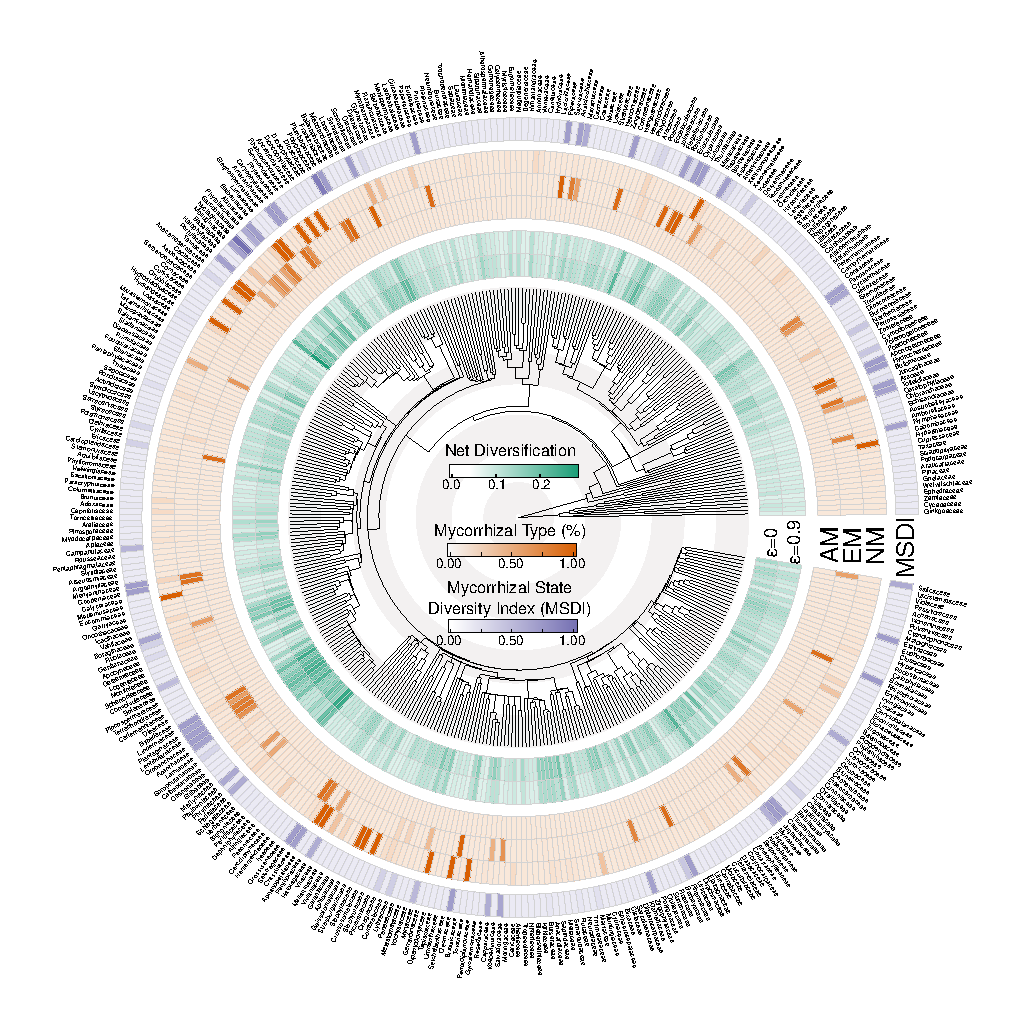
\includegraphics{../output/tree_fig/phylo_genus_final_resized.pdf}
\caption{Family-level, time-calibrated phylogeny for the 106 seed plant
families included in the analyses. For each family, the proportion of
species within each mycorrhizal type is represented in the yellow-to-red
boxes, AM: Arbuscular mycorrhiza, EM: Ectomycorrhiza and NM:
non-mycorrhizal. The mycorrhizal diversity index (MDI) is represented in
the green boxes and the diversification rate (r) is shown in the purple
boxes. To illustrate the timescale of the phylogeny, the width of
concentric white and gray circles represents 100 million years.}
\end{figure}

\begin{figure}
\centering
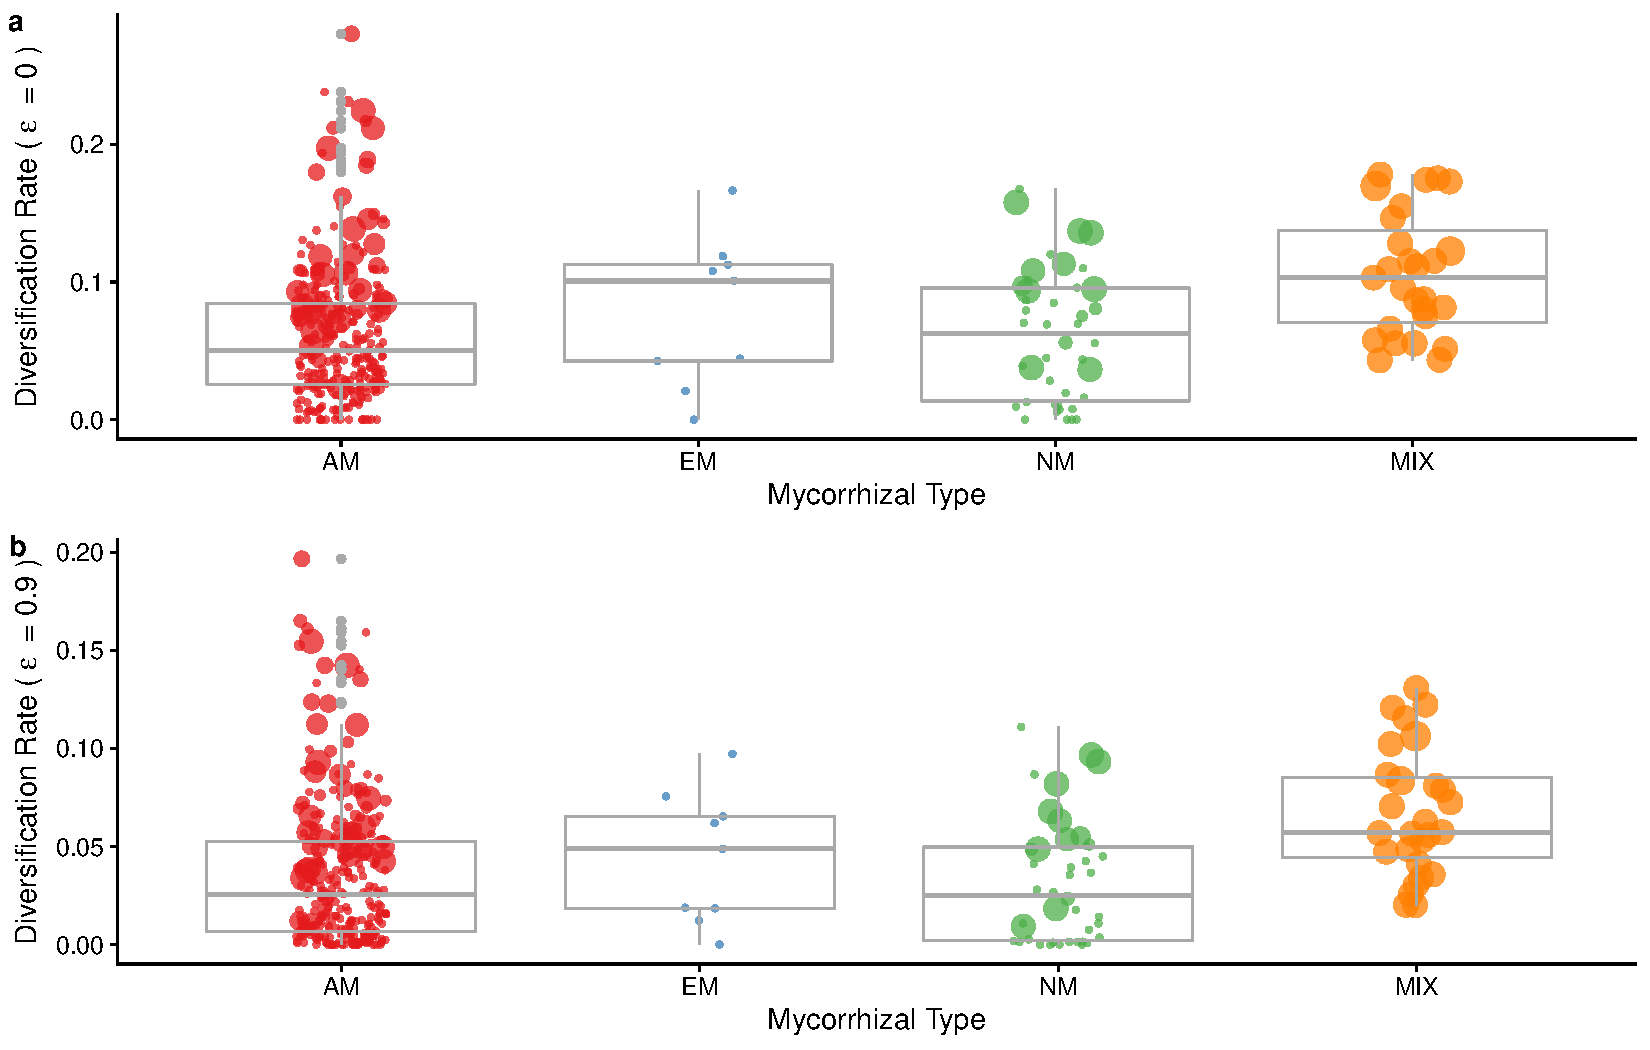
\includegraphics{../output/figs/boxplots_netdiv_myctype.pdf}
\caption{Relationship between mycorrhizal type and diversification
rates. a) diversification rate estimated with \(\epsilon\) (relative
extinction fraction) = 0 and b) diversification rate estimated with
\(\epsilon\) = 0.9. AM: Arbuscular mycorrhiza, EM: Ectomycorrhiza, NM:
non-mycorrhizal and MIX (families with no dominance of any specific
mycorrhizal association).}
\end{figure}

\begin{figure}
\centering
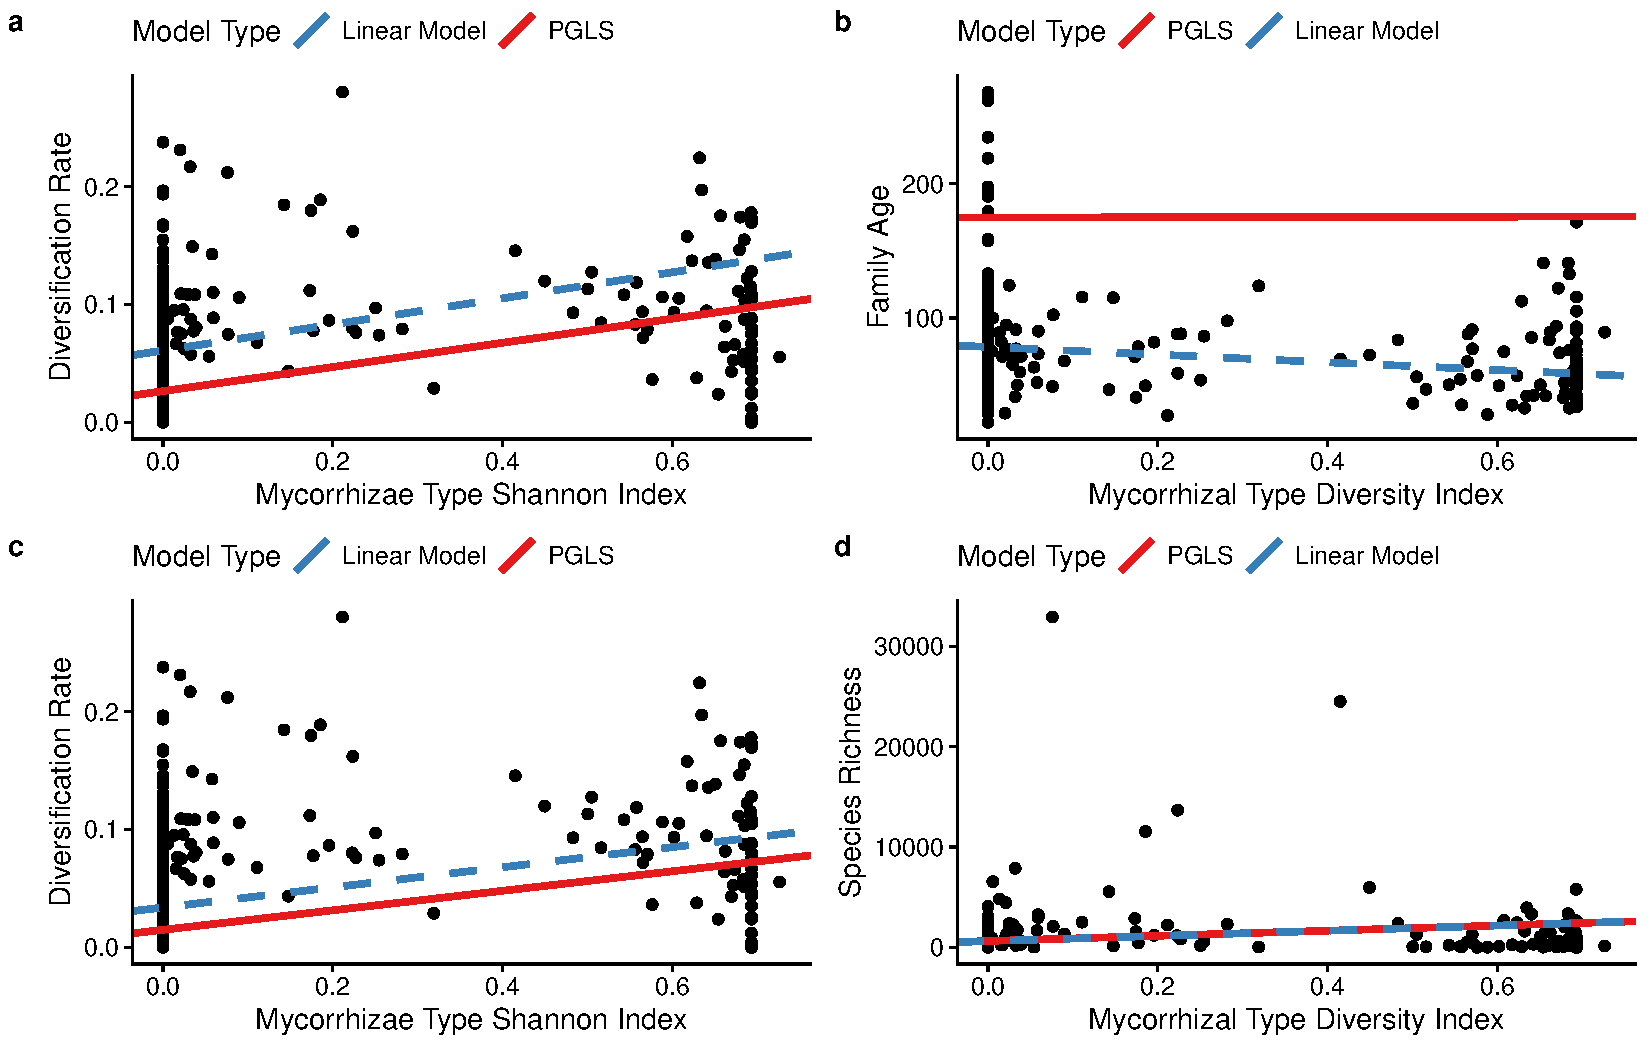
\includegraphics{../output/figs/scatterplots_lm_pgls_stem.pdf}
\caption{Scatterplots showing the relationship between mycorrhizal
diversity index and diversification rates, species richness and age
family. The red and blue lines indicate the results of a linear model
and a phylogenetic generalized least squares (PGLS) fit, respectively.
b) and d) show the correlation between observed values of
diversification rate and estimated values obtained from the PGLS (red
line represents the perfect fit).}
\end{figure}


\end{document}
